% questions.tex —— 1996 年·上海卷·文史类 · 题目内容片段（无答案）
% 由 tools/generate_projects.py 依来源总账自 1996/1996_数学真题_上海文史_试题.md 生成，勿手改（改源 MD 后重跑）


\gkpart{数学试卷}

\begin{gktip}
\textbf{来源说明}：本题面依据固定来源 PDF 逐题转录，扫描件共 8 页，印刷页码 83—90。原卷载明 24 道试题、满分 150 分（选择题 8 题，满分 24 分，每题 3 分；填空题 10 题，满分 40 分，每空格 4 分；解答题 6 题，满分 86 分），并设 A1/B1、A2/B2 对应选做组；具体组别和计分规则按原卷保留。固定 PDF 所载答案及评分解析另见答案要点、解析正文。来源出版者与官方性尚未核实，故只称“固定来源所载”，不宣称为已核实的官方版本。本稿待独立复核。

\textbf{图形说明}：第 8、20、21、23 题的图形以 TikZ 按扫描件可辨认的结构关系重绘；曲线比例、空间投影和长度不作为额外数学条件。
\end{gktip}

\begin{question}
\gkti{1}已知集合

\nopagebreak[4]
\[
M=\{(x,y)\mid x+y=2\},\qquad N=\{(x,y)\mid x-y=4\},
\]

那么集合 $M\cap N$ 为\mbox{（　　）}。

（A）$x=3,\ y=-1$　　（B）$(3,-1)$　　（C）$\{3,-1\}$　　（D）$\{(3,-1)\}$

\end{question}
\begin{question}
\gkti{2}在下列各区间中，函数 $y=\sin\left(x+\dfrac{\pi}{4}\right)$ 的单调递增区间是\mbox{（　　）}。

（A）$\left[\dfrac{\pi}{2},\pi\right]$　　（B）$\left[0,\dfrac{\pi}{4}\right]$　　（C）$[-\pi,0]$　　（D）$\left[\dfrac{\pi}{4},\dfrac{\pi}{2}\right]$

\end{question}
\begin{question}
\gkti{3}过点 $(4,0)$ 和点 $(0,3)$ 的直线的倾斜角为\mbox{（　　）}。

（A）$\arctan\dfrac{3}{4}$　　（B）$\pi-\arctan\dfrac{3}{4}$　　（C）$\arctan\left(-\dfrac{3}{4}\right)$　　（D）$\pi-\arctan\left(-\dfrac{3}{4}\right)$

\end{question}
\begin{question}
\gkti{4}在下列命题中，真命题是\mbox{（　　）}。

（A）若直线 $m,n$ 都平行于平面 $\alpha$，则 $m\parallel n$。

（B）设 $\alpha-l-\beta$ 是直二面角。若直线 $m\perp l$，则 $m\perp\beta$。

（C）若直线 $m,n$ 在平面 $\alpha$ 内的射影依次是一个点和一条直线，且 $m\perp n$，则 $n$ 在 $\alpha$ 内或 $n$ 与 $\alpha$ 平行。

（D）设 $m,n$ 是异面直线。若 $m$ 与平面 $\alpha$ 平行，则 $n$ 与 $\alpha$ 相交。

\end{question}
\begin{question}
\gkti{5}将椭圆

\nopagebreak[4]
\[
\dfrac{x^2}{25}+\dfrac{y^2}{9}=1
\]

绕其左焦点按逆时针方向旋转 $90^\circ$ 后所得的椭圆方程是\mbox{（　　）}。

（A）$\dfrac{(x+4)^2}{25}+\dfrac{(y-4)^2}{9}=1$　　（B）$\dfrac{(x+4)^2}{25}+\dfrac{(y+4)^2}{9}=1$

（C）$\dfrac{(x+4)^2}{9}+\dfrac{(y-4)^2}{25}=1$　　（D）$\dfrac{(x+4)^2}{9}+\dfrac{(y+4)^2}{25}=1$

\end{question}
\begin{question}
\gkti{6}若 $y=f(x)$ 是定义在 $\mathbb R$ 上的函数，则 $y=f(x)$ 为奇函数的一个充要条件是\mbox{（　　）}。

（A）$f(0)=0$　　（B）对任意的 $x\in\mathbb R$，$f(x)=0$ 都成立

（C）存在某一 $x_0\in\mathbb R$，使得 $f(x_0)+f(-x_0)=0$

（D）对任意的 $x\in\mathbb R$，$f(x)+f(-x)=0$

\end{question}
\begin{question}
\gkti{7}如果 $\log_a3>\log_b3>0$，那么 $a,b$ 间的关系是\mbox{（　　）}。

（A）$0<b<a<1$　　（B）$0<a<b<1$　　（C）$1<b<a$　　（D）$1<a<b$

\Needspace{0.4\textheight}
\end{question}
\begin{question}
\gkti{8}在下列图象中，二次函数 $y=ax^2+bx$ 与指数函数 $y=\left(\dfrac{b}{a}\right)^x$ 的图象只可能是\mbox{（　　）}。
\nopagebreak[4]
\begin{center}% 固定来源 PDF 印刷页 84 第 8 题四组选项图象的矢量示意重绘。
% 选项相对形状、抛物线开口/过原点关系和指数曲线过 (0,1) 按原图描绘；曲线比例仅为示意。
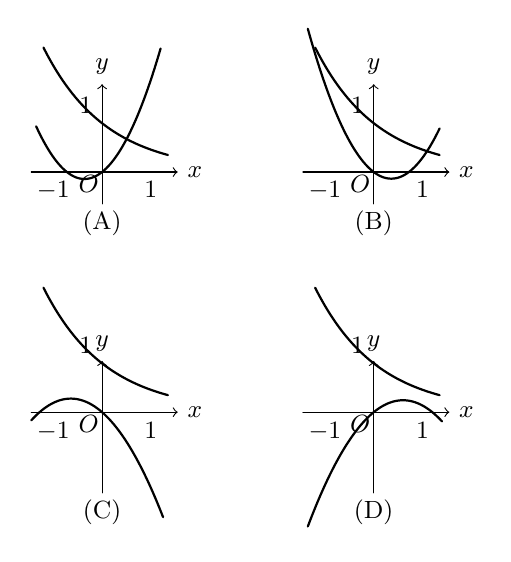
\begin{tikzpicture}[x=.62cm,y=.62cm,font=\small,line cap=round,line join=round]
  % (A) upward parabola with its second zero left of the origin.
  \begin{scope}
    \draw[->] (-1.45,0)--(1.55,0) node[right] {$x$};
    \draw[->] (0,-.65)--(0,1.8) node[above] {$y$};
    \draw[thick,domain=-1.35:1.2,samples=70,variable=\x]
      plot (\x,{1.1*\x*(\x+.72)});
    \draw[thick,domain=-1.2:1.35,samples=70,variable=\x]
      plot (\x,{exp(-.78*\x)});
    \node[below left,inner sep=1pt] at (0,0) {$O$};
    \node[below] at (-1,0) {$-1$}; \node[below] at (1,0) {$1$};
    \node[above left] at (0,1) {$1$}; \node at (0,-1.05) {(A)};
  \end{scope}
  % (B) upward parabola with its second zero right of the origin.
  \begin{scope}[xshift=3.45cm]
    \draw[->] (-1.45,0)--(1.55,0) node[right] {$x$};
    \draw[->] (0,-.65)--(0,1.8) node[above] {$y$};
    \draw[thick,domain=-1.35:1.35,samples=70,variable=\x]
      plot (\x,{1.05*\x*(\x-.72)});
    \draw[thick,domain=-1.2:1.35,samples=70,variable=\x]
      plot (\x,{exp(-.78*\x)});
    \node[below left,inner sep=1pt] at (0,0) {$O$};
    \node[below] at (-1,0) {$-1$}; \node[below] at (1,0) {$1$};
    \node[above left] at (0,1) {$1$}; \node at (0,-1.05) {(B)};
  \end{scope}
  % (C) downward parabola with its second zero left of the origin.
  \begin{scope}[yshift=-3.05cm]
    \draw[->] (-1.45,0)--(1.55,0) node[right] {$x$};
    \draw[->] (0,-1.65)--(0,1.05) node[above] {$y$};
    \draw[thick,domain=-1.45:1.25,samples=70,variable=\x]
      plot (\x,{-.68*\x*(\x+1.28)});
    \draw[thick,domain=-1.2:1.35,samples=70,variable=\x]
      plot (\x,{exp(-.78*\x)});
    \node[below left,inner sep=1pt] at (0,0) {$O$};
    \node[below] at (-1,0) {$-1$}; \node[below] at (1,0) {$1$};
    \node[above left] at (0,1) {$1$}; \node at (0,-2.05) {(C)};
  \end{scope}
  % (D) downward parabola with its second zero right of the origin.
  \begin{scope}[xshift=3.45cm,yshift=-3.05cm]
    \draw[->] (-1.45,0)--(1.55,0) node[right] {$x$};
    \draw[->] (0,-1.65)--(0,1.05) node[above] {$y$};
    \draw[thick,domain=-1.35:1.4,samples=70,variable=\x]
      plot (\x,{-.68*\x*(\x-1.2)});
    \draw[thick,domain=-1.2:1.35,samples=70,variable=\x]
      plot (\x,{exp(-.78*\x)});
    \node[below left,inner sep=1pt] at (0,0) {$O$};
    \node[below] at (-1,0) {$-1$}; \node[below] at (1,0) {$1$};
    \node[above left] at (0,1) {$1$}; \node at (0,-2.05) {(D)};
  \end{scope}
\end{tikzpicture}
\end{center}
\nopagebreak[4]
\end{question}
\begin{question}
\gkti{9}方程

\nopagebreak[4]
\[
\log_2(9^x-5)=\log_2(3^x-2)+2
\]

的解是 $x=\underline{\qquad\qquad}$。

\end{question}
\begin{question}
\gkti{10}函数

\nopagebreak[4]
\[
y=\dfrac{1}{\sqrt{\log_{1/2}(2-x)}}
\]

的定义域是 $\underline{\qquad\qquad}$。

\end{question}
\begin{question}
\gkti{11}方程

\nopagebreak[4]
\[
\sin\left(x-\dfrac{\pi}{3}\right)=\dfrac{\sqrt{2}}{2}
\]

在 $[0,\pi]$ 上的解是 $x=\underline{\qquad\qquad}$。

\end{question}
\begin{question}
\gkti{12}函数 $y=x^{-2}\ (x<0)$ 的反函数是 $y=\underline{\qquad\qquad}$。

\end{question}
\begin{question}
\gkti{13}与圆 $(x-2)^2+y^2=1$ 外切，且与 $y$ 轴相切的动圆圆心 $P$ 的轨迹方程为 $\underline{\qquad\qquad}$。

\end{question}
\begin{question}
\gkti{14}在 $(1+x)^2(1-x)^4$ 的展开式中，$x^3$ 的系数是 $\underline{\qquad\qquad}$（结果用数值表示）。

\end{question}
\gkpart{选做题：A1 组与 B1 组}

考生可从下列两组（A1 组和 B1 组）中选做一组试题；其中 A1 组适合非试点学校考生，B1 组适合试点学校考生。

\begin{question}
\gkti{15}本题分 A1、B1 两种选做版本。

\textbf{A1 组：} 已知 $O(0,0)$ 和 $A(6,3)$ 两点，若点 $P$ 在直线 $OA$ 上，且 $\dfrac{OP}{PA}=\dfrac12$，又 $P$ 是线段 $OB$ 的中点，则点 $B$ 的坐标是 $\underline{\qquad\qquad}$。

\textbf{B1 组：} 已知向量 $\vec a+\vec b=2\vec i-8\vec j$，$\vec a-\vec b=-8\vec i+16\vec j$，那么 $\vec a\cdot\vec b=\underline{\qquad\qquad}$。

\end{question}
\begin{question}
\gkti{16}本题分 A1、B1 两种选做版本。

\Needspace{5\baselineskip}
\textbf{A1 组：} 平移坐标轴将抛物线

\nopagebreak[4]
\[
4x^2-8x+y+5=0
\]

化为标准方程 $x'^2=ay'\ (a\ne0)$，则新坐标系的原点在原坐标系中的坐标是 $\underline{\qquad\qquad}$。

\Needspace{5\baselineskip}
\textbf{B1 组：}

\nopagebreak[4]
\[
\lim_{x\to2}\left(\dfrac{4}{x^2-4}-\dfrac{1}{x-2}\right)=\underline{\qquad\qquad}\text{。}
\]

\end{question}
\begin{question}
\gkti{17}本题分 A1、B1 两种选做版本。有 8 本互不相同的书，其中数学书 3 本、外文书 2 本、其它书 3 本。

\textbf{A1 组：} 若将这些书排成一列放在书架上，则数学书恰好排在一起，外文书也恰好排在一起的排法共有 $\underline{\qquad\qquad}$ 种（结果用数值表示）。

\textbf{B1 组：} 若将这些书随机地排成一列放在书架上，则数学书恰好排在一起、外文书也恰好排在一起的概率为 $\underline{\qquad\qquad}$（结果用分数表示）。

\end{question}
\begin{question}
\gkti{18}本题分 A1、B1 两种选做版本。

\textbf{A1 组：} 把半径为 $3\text{ cm}$、中心角为 $\dfrac{2\pi}{3}$ 的扇形卷成一个圆锥形容器，这个容器的体积为 $\underline{\qquad\qquad}\text{ cm}^3$（结果保留 $\pi$）。

\textbf{B1 组：} 某人有 10 万元，准备用于投资房地产或购买股票。如果根据下面的盈利表进行决策，那么决策方案是 $\underline{\qquad\qquad}$。

\begin{center}
\begin{tabular}{lrrr}
\toprule
自然状况 & 盈利概率 & 购买股票（万元） & 投资房地产（万元） \\
\midrule
巨大成功 & $0.3$ & $10$ & $8$ \\
中等成功 & $0.5$ & $3$ & $4$ \\
失败 & $0.2$ & $-5$ & $-4$ \\
\bottomrule
\end{tabular}
\end{center}

\end{question}
\gkpart{解答题}

\begin{question}
\gkti{19}（本题满分 10 分）已知

\nopagebreak[4]
\[
\sin\left(\dfrac{\pi}{4}+\alpha\right)\sin\left(\dfrac{\pi}{4}-\alpha\right)=\dfrac16,\qquad \alpha\in\left(\dfrac\pi2,\pi\right),
\]

求 $\sin4\alpha$ 的值。

\Needspace{0.4\textheight}
\end{question}
\begin{question}
\gkti{20}（本题满分 10 分）本题共有 2 个小题，第 1 小题满分 6 分，第 2 小题满分 4 分。在如图所示的直角坐标系中，一运动物体经过点 $A(0,9)$，其轨迹方程为 $y=ax^2+c\ (a<0)$，$D=(6,7)$ 为 $x$ 轴上的给定区间。

（1） 为使物体落在 $D$ 内，求 $a$ 的取值范围；

（2） 若物体运动时又经过点 $P(2,8.1)$，问它能否落在 $D$ 内？并说明理由。
\nopagebreak[4]
\begin{center}% 固定来源 PDF 印刷页 85 第 20 题坐标图的示意重绘。
% 标出 A、P 与 x 轴区间 D=(6,7)；抛物线仅示意一条满足题中数值关系的轨迹。
\begin{tikzpicture}[x=.48cm,y=.40cm,font=\small,line cap=round,line join=round]
  \draw[->] (-1,0)--(8,0) node[right] {$x$};
  \draw[->] (0,-1.4)--(0,10) node[above] {$y$};
  \draw[thick,domain=-6.2:6.4,samples=100,variable=\x]
    plot (\x,{9-.225*\x*\x});
  \fill (0,9) circle (1.8pt) node[above left] {$A$};
  \fill (2,8.1) circle (1.8pt) node[above right] {$P$};
  \draw[thick] (6,0)--(7,0);
  \draw (6,.15)--(6,-.15) node[below=2pt] {$6$};
  \draw (7,.15)--(7,-.15) node[below=2pt] {$7$};
  \node[below=9pt] at (6.5,0) {$D=(6,7)$};
  \node[left] at (0,9) {$9$};
  \node[below left,inner sep=1pt] at (0,0) {$O$};
\end{tikzpicture}
\end{center}
\nopagebreak[4]
\Needspace{0.4\textheight}
\end{question}
\begin{question}
\gkti{21}（本题满分 14 分）本题共有 3 个小题，第 1 小题满分 4 分，第 2、3 小题各满分 5 分。如图，在二面角 $\alpha-l-\beta$ 中，$A,B\in\alpha$，$C,D\in l$，$ABCD$ 为矩形，$P\in\beta$，$PA\perp\alpha$，且 $PA=AD$。$M,N$ 依次是 $AB,PC$ 的中点。

（1） 求二面角 $\alpha-l-\beta$ 的大小；

（2） 求证：$MN\perp AB$；

（3） 求异面直线 $PA$ 与 $MN$ 所成角的大小。
\nopagebreak[4]
\begin{center}% 固定来源 PDF 印刷页 85 第 21 题原图结构示意重绘。
% 两平面相交于 l，矩形 ABCD 位于 alpha，P 属于 beta 且 PA 垂直 alpha；空间投影不代表长度比例。
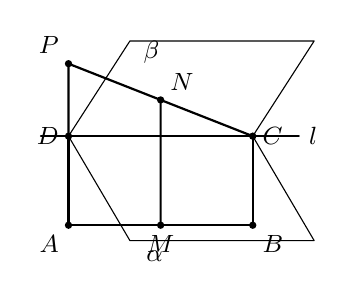
\begin{tikzpicture}[scale=.78,font=\small,line cap=round,line join=round]
  \coordinate (D) at (1,0);
  \coordinate (C) at (4,0);
  \coordinate (A) at (1,-1.45);
  \coordinate (B) at (4,-1.45);
  \coordinate (P) at (1,1.18);
  \coordinate (M) at (2.5,-1.45);
  \coordinate (N) at (2.5,.59);
  % Plane alpha and beta share the line l=DC.
  \draw[thin] (D)--(C)--(5,-1.7)--(2,-1.7)--cycle;
  \draw[thin] (D)--(C)--(5,1.55)--(2,1.55)--cycle;
  \draw[thick] (.55,0)--(4.75,0) node[right] {$l$};
  \node at (2.4,-1.95) {$\alpha$};
  \node at (2.35,1.37) {$\beta$};
  % Rectangle and the given point/segments.
  \draw[thick] (A)--(B)--(C)--(D)--cycle;
  \draw[thick] (P)--(A) (P)--(C) (M)--(N);
  \fill (A) circle (1.7pt) node[below left] {$A$};
  \fill (B) circle (1.7pt) node[below right] {$B$};
  \fill (C) circle (1.7pt) node[right] {$C$};
  \fill (D) circle (1.7pt) node[left] {$D$};
  \fill (P) circle (1.7pt) node[above left] {$P$};
  \fill (M) circle (1.7pt) node[below] {$M$};
  \fill (N) circle (1.7pt) node[above right] {$N$};
\end{tikzpicture}
\end{center}
\nopagebreak[4]
\end{question}
\gkpart{选做题：A2 组与 B2 组}

考生可从下列两组（A2 组和 B2 组）中选做一组试题；其中 A2 组适合非试点学校考生，B2 组适合试点学校考生。

\begin{question}
\gkti{22}（本题满分 16 分）本题有 A2、B2 两种选做版本。A2 组本题共有 3 个小题，第 1、3 小题各满分 6 分，第 2 小题满分 4 分。设

\nopagebreak[4]
\[
z=a+bi\quad(a,b\in\mathbb R,\ b\ne0,\ i\text{ \text{为虚数单位}}),\qquad w=z+\dfrac1z
\]

是实数，且 $-1<w<2$。

（1） 求 $|z|$ 的值及 $z$ 的实部的取值范围；

（2） 设 $u=\dfrac{1-z}{1+z}$，求证：$u$ 为纯虚数；

（3） 求 $w-u^2$ 的最小值。

\textbf{B2 组：} 本题共有 3 个小题，第 1 小题满分 4 分，第 2 小题满分 5 分，第 3 小题满分 7 分。已知 $A(-1,2)$ 为抛物线 $C:y=2x^2$ 上的点，直线 $l_1$ 过点 $A$，且与抛物线 $C$ 相切。直线 $l_2:x=a\ (a\ne-1)$ 交抛物线 $C$ 于点 $B$，交直线 $l_1$ 于点 $D$。

（1） 求直线 $l_1$ 的方程；

（2） 设 $\triangle ABD$ 的面积为 $S_1$，求 $|BD|$ 及 $S_1$ 的值；

（3） 设由抛物线 $C$、直线 $l_1,l_2$ 所围成的图形的面积为 $S_2$，求证：$S_1:S_2$ 的值为与 $a$ 无关的常数。

\Needspace{0.4\textheight}
\end{question}
\begin{question}
\gkti{23}（本题满分 18 分）第 1、2 小题各满分 4 分，第 3 小题满分 10 分。已知双曲线 $S$ 的两条渐近线过坐标原点，且与以点 $A(\sqrt2,0)$ 为圆心、$1$ 为半径的圆相切；双曲线 $S$ 的一个顶点 $A'$ 与点 $A$ 关于直线 $y=x$ 对称。

（1） 求双曲线 $S$ 的方程；

（2） 设直线 $l$ 过点 $A$，斜率为 $1$。在双曲线 $S$ 的上支上求点 $B$，使其与直线 $l$ 的距离为 $\sqrt2$；

（3） 求双曲线 $S$ 上到直线 $l:y=\dfrac{2\sqrt5}{5}(x-\sqrt2)$ 的距离为 $\sqrt2$ 的点的个数。
\nopagebreak[4]
\begin{center}% 固定来源 PDF 印刷页 86 第 23 题双曲线、渐近线及圆的结构示意重绘。
% 双曲线、圆心 A、圆半径和渐近线按题面关系作图；示意不添加未给定条件。
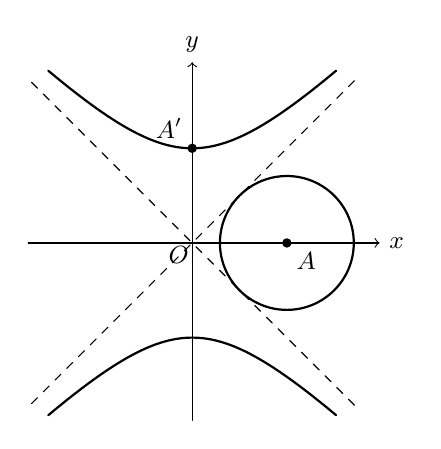
\begin{tikzpicture}[x=.85cm,y=.85cm,font=\small,line cap=round,line join=round]
  \draw[->] (-2.45,0)--(2.8,0) node[right] {$x$};
  \draw[->] (0,-2.65)--(0,2.7) node[above] {$y$};
  \draw[dashed] (-2.4,-2.4)--(2.5,2.5);
  \draw[dashed] (-2.4,2.4)--(2.5,-2.5);
  \draw[thick,domain=-2.15:2.15,samples=100,variable=\x]
    plot (\x,{sqrt(\x*\x+2)});
  \draw[thick,domain=-2.15:2.15,samples=100,variable=\x]
    plot (\x,{-sqrt(\x*\x+2)});
  \draw[thick] (1.4142,0) circle (1);
  \fill (0,1.4142) circle (1.7pt) node[above left] {$A'$};
  \fill (1.4142,0) circle (1.7pt) node[below right] {$A$};
  \node[below left,inner sep=1pt] at (0,0) {$O$};
\end{tikzpicture}
\end{center}
\nopagebreak[4]
\end{question}
\begin{question}
\gkti{24}（本题满分 18 分）本题共有 2 个小题，第 1 小题满分 6 分，第 2 小题满分 12 分。设 $A_n$ 为数列 $\{a_n\}$ 的前 $n$ 项和，

\nopagebreak[4]
\[
A_n=\dfrac{3}{2}(a_n-1)\quad(n\in\mathbb N),
\]

\Needspace{5\baselineskip}
数列 $\{b_n\}$ 的通项公式为

\nopagebreak[4]
\[
b_n=4n+3\quad(n\in\mathbb N)\text{。}
\]

（1） 求数列 $\{a_n\}$ 的通项公式；

（2） 若 $d\in\{a_1,a_2,a_3,\ldots\}\cap\{b_1,b_2,b_3,\ldots\}$，则称 $d$ 为数列 $\{a_n\}$ 与 $\{b_n\}$ 的公共项。将这两个数列的公共项按它们在原数列中的先后顺序排成一个新数列 $\{d_n\}$，证明数列 $\{d_n\}$ 的通项公式为 $d_n=3^{2n+1}\ (n\in\mathbb N)$。

\end{question}